\chapter{Introduction}
\label{chp:introduction}

Development of complex systems requires an efficient way for engineers to ensure the correctness of the developed software. Domain Specific Modeling (DSM) can, through automatic code generation and block-diagram visualizations, significantly reduce the risk of faulty applications, and enable engineers to work more effectively. In safety-critical development processes however, DSM can only be used without subsequent manual verification, if the DSM tools work correctly. This can either be achieved through time intensive qualified software development processes, which ensure accurate and reliable visualization of DSM through the tool itself, or through the use of unverified DSM tools followed by the subsequent use of a small visualization verification tool to ensure the correctness of the application.\\
In low-cost projects with high safety requirements, a cost-effective qualification method is crucial, highlighting the potential of the latter approach for a qualifiable graphical editing tool for use in DSM.\\
\newline
The Institute for Aircraft Systems is currently developing a way for avionic models to be developed inside a web-based graphical model editor called "eXtensible Graphical EMOF Editor" or "XGEE".\\
XGEE uses three kinds of "tokens" within three distinct editors to visualize avionic models. They are:
\begin{itemize}
    \item signals
    \item vertices
    \item text labels
\end{itemize}
\begin{figure}[h]
    \centering
    % First image
    \begin{subfigure}{0.3\textwidth}
        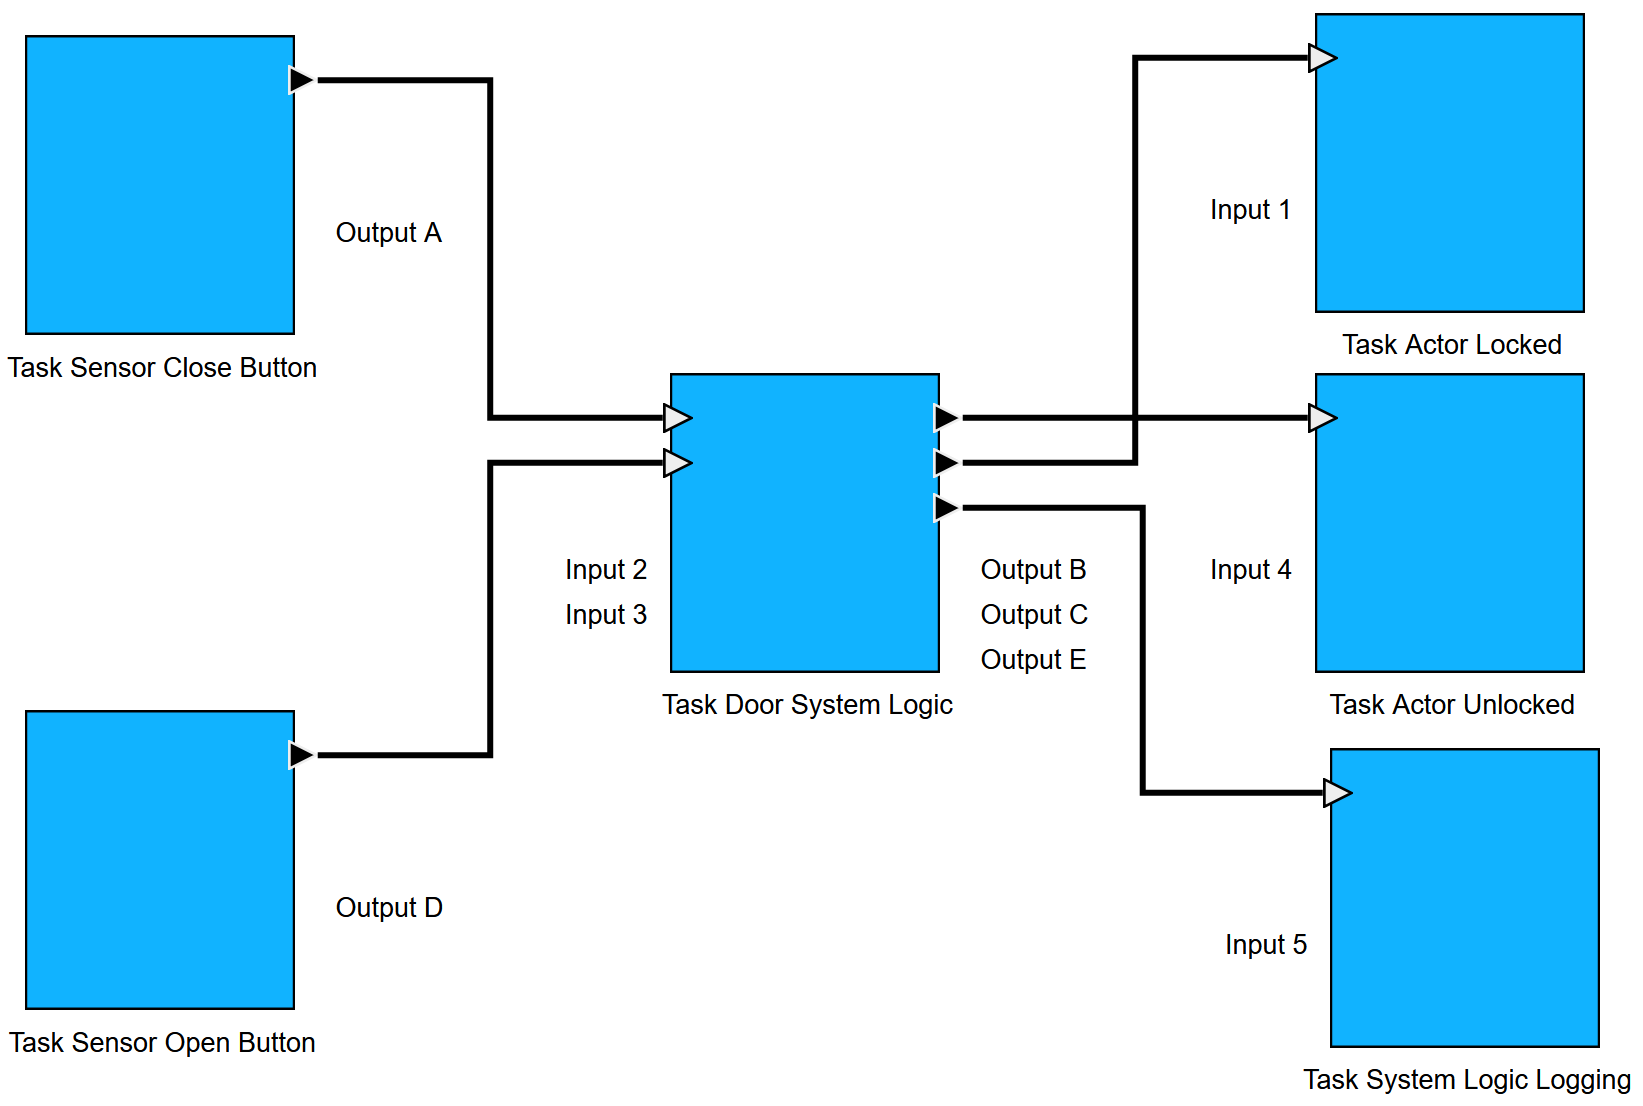
\includegraphics[width=\linewidth]{Pictures/functions_editor.png}
        \caption{Functions editor}
        \label{fig_functions_editor_en}
    \end{subfigure}
    \hfill
    % Second image
    \begin{subfigure}{0.3\textwidth}
        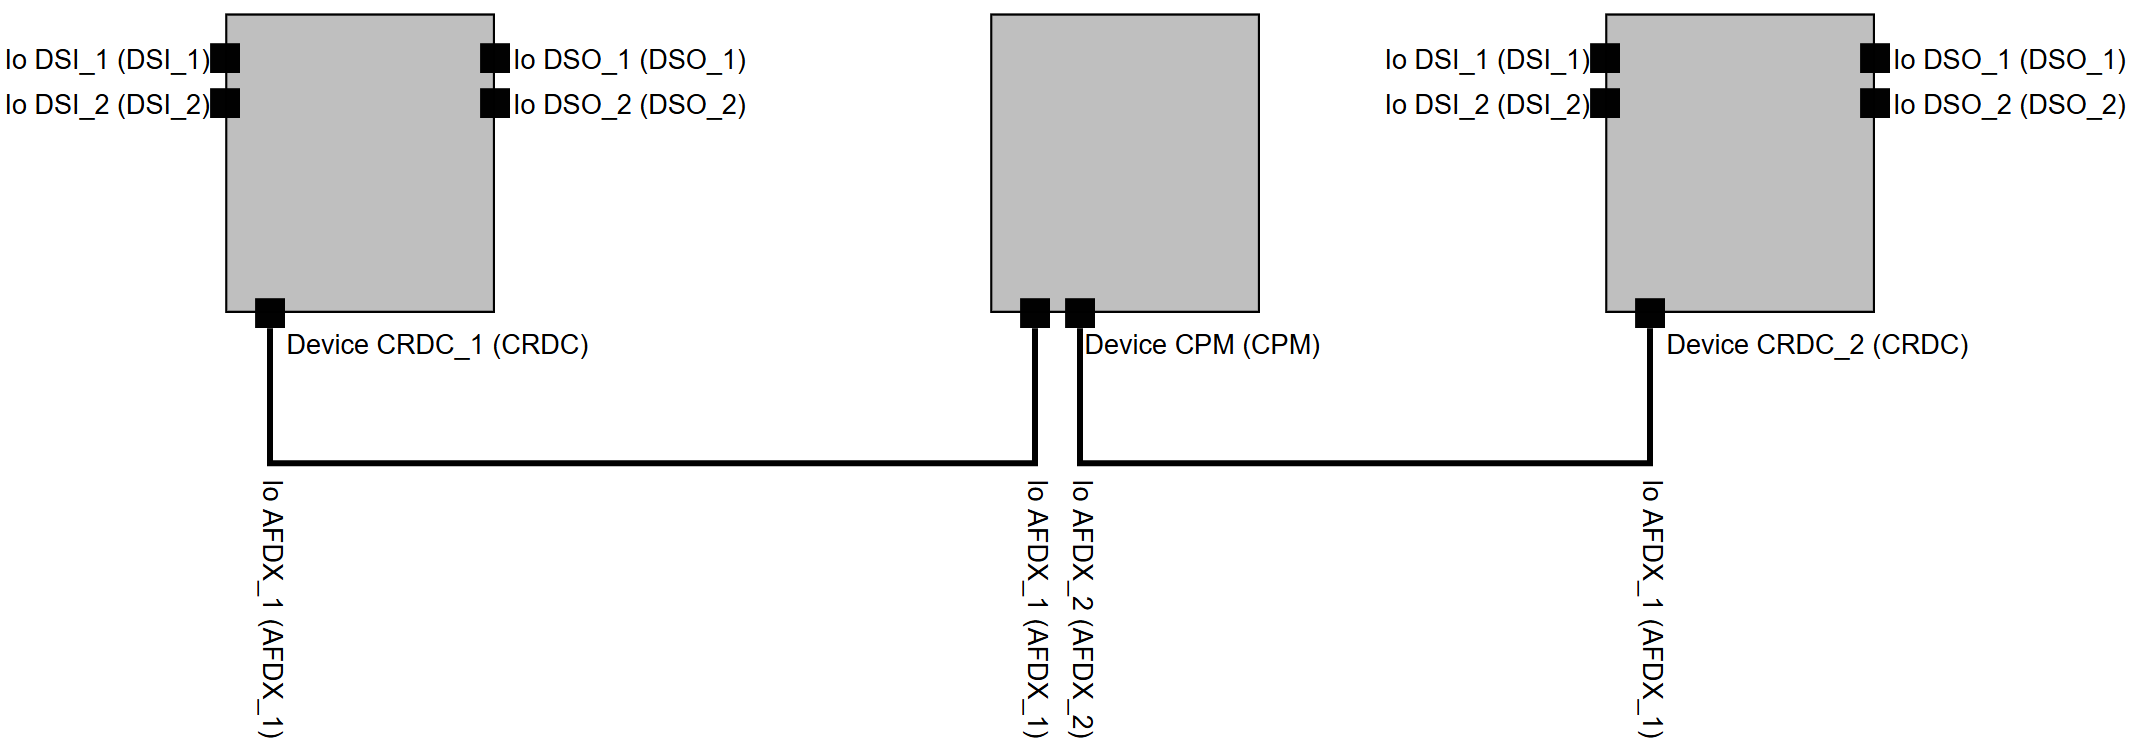
\includegraphics[width=\linewidth]{Pictures/hardware_editor.png}
        \caption{Hardware editor}
        \label{fig_hardware_editor_en}
    \end{subfigure}
    \hfill
    % Third image
    \begin{subfigure}{0.3\textwidth}
        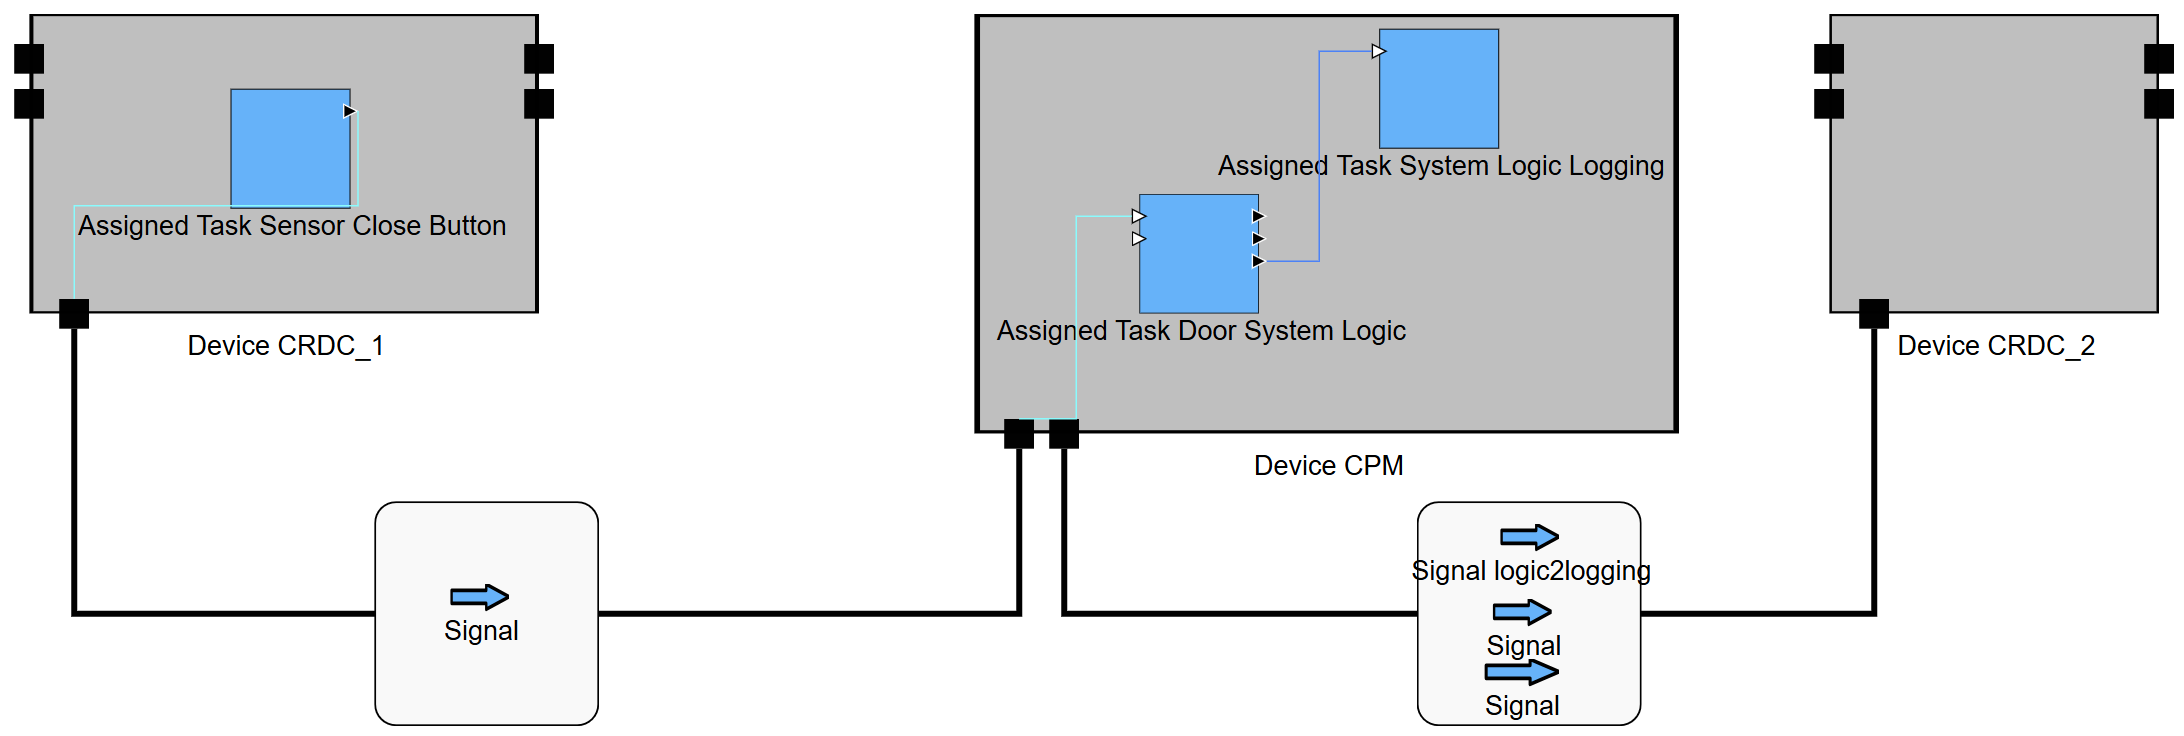
\includegraphics[width=\linewidth]{Pictures/allocations_editor.png}
        \caption{Allocations editor}
        \label{fig_allocations_editor_en}
    \end{subfigure}

    \caption{Functions- Hardware- and Allocations editors}
    \label{fig_editors_en}
\end{figure}
This paper builds upon the work of \cite{ar_prof_paper} to automate the verification process within XGEE by tokenizing a screenshot from within the editor. To recognize and process the screenshot data, methods from the "Open Computer Vision" (OpenCV) library are being used.\\
By rebuilding a model from the recognized tokens and comparing it to the original, visualization errors become apparent and can be indicated to the user.
Common visualization errors include:
\begin{itemize}
    \item unclear signal intersections
    \item signals being obscured by blocks
    \item text labels being obscured by signals or blocks
    \item blocks being scaled down to the point of disappearing
    \item blocks obscuring other blocks
\end{itemize}

\section{State of the Art}
\label{sec_state_of_the_art}

The visualization verification tool in \cite{ar_prof_paper} could preprocess an automatic screenshot, tokenize edges, vertices and labels, rebuild a model based on the recognized tokens and compare the recognized model with the original.\\
To preprocess the screenshot, the XGEE window is found by searching for the distinct colors of the XGEE title- and status bar and defining the bounding box of the actual block diagram. The grey pixels of the grid are replaced with white, since they are not relevant for the model tokenization.

The vertex detection algorithm was able to detect blue function containers, inputs and outputs with great accuracy, as long as they did not exceed the size limit set by the used template.
The original edge detection algorithm was able to detect edges that went from left to right and from top to bottom with high accuracy. 
The original text detection was using PyTesseract and worked very well, if the text was oriented properly.

\section{Computer Vision}
    
\section{Domain Specific Modeling}

\section{XGEE}

\section{Python}

\section{OpenCV}